% !TEX root = ../main.tex

% Local Variables:
% TeX-master: "../main"
% End:
% chktex-file 26

%%%%%%%%%%%%%%%%%%%%%%%%%%%%%%% Header %%%%%%%%%%%%%%%%%%%%%%%%%%%%%%%%%%%%%%%%%%%%
\begin{minipage}[l]{0.42\textwidth}
    
\includegraphics[width=1\textwidth]{img/logo-UNAMBA.png}
\end{minipage}
\hfill
\begin{minipage}[c]{0.5\textwidth}
    \begin{flushright}
	\large{\textbf{Unidad \#2}}\\
	\large{Lectures on Física I}\\
	\large{24 de Julio del 2025. Haquira, Apurimac}\\
        % \large{\textbf{Student:} Huallpa Aimituma Josué David}
    \end{flushright}
\end{minipage}
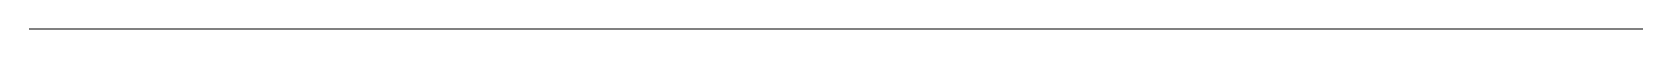
\begin{tikzpicture}
    \draw[gray,thick] (-6.5,0)--(14,0);
\end{tikzpicture}


 %%%%%%%%%%%%%%%%%%%%%%%% INICIO DEL CONTENIDO EN DOS COLUMNAS %%%%%%%%%%%%%%%%%%%%%

 \begin{multicols}{2}
     \begin{center}
         \LARGE{\textbf{Capítulo IV: Cinemática del punto}}\\	
         \vspace{0.2cm}
         % \Large {Lecturers Esteban Chalbaud \& Daniel Galviz} \\
         % \large{Teaching Assistant: Mauricio Gamonal \& Irvin Martínez}\\
         % \large{PhysicsLatam.com}\\
         % \vspace{0.2cm}
         \large{Fecha de entrega: 07 Agosto 2025, 5:59 pm (GMT-4)}\\
         % \vspace{0.2cm}
         \large{— Evaluación Parcial 2 —}
     \end{center}
    
    %%%%%%%%%%%%%%%%%%%%%%%%%%%%excercise%%%%%%%%%%%%%%%%%%%%%%%%%%%%%%%%%%%%%%%%
     \begin{excercise}[][][]{ex:k0}{
        \textbf{(3 pts.)} Una partícula se mueve en el plano $xy$ con aceleración constante.        
        \begin{equation*}
            \vec{a}=6\vec{\imath}+4\vec{\jmat}
        \end{equation*}
        En el instante $t=0$, la velocidad es cero, y el vector posición esta dado por:
        \begin{equation*}
            \vec{r}=10\vec{\imath}
        \end{equation*}
        \begin{itemize}
            \item[a)] Hallar el vector velocidad y vector posición de la particula en un instante cualquiera $t$.
            \item[b)] Elimine el tiempo y obtenga la ecuación cartesiana de la trayectoria en el plano $xy$.
            \item[c)] Halle el vector velocidad media y la rapidez media entre $t=1\,\mathrm{s}$ y $t=3\,\mathrm{s}$.
            \item[d)] Represente gráficamente la trayectoria en el plano $xy$. La ecuación de la trayectoria encontrada en el inciso (b) corresponde a una recta. Calcule su pendiente y encuentre el ángulo formado por la recta con el eje de las absisas. Para grafica puede tabular los valores de $(x,y)$ del vector posición para distintos $t$, como (t=1, 2, 3, 4, ...). Traze la trayectoria a mano. 
        \end{itemize}
         }
     \end{excercise} 

   
    %%%%%%%%%%%%%%%%%%%%%%%%%%%%excercise%%%%%%%%%%%%%%%%%%%%%%%%%%%%%%%%%%%%%%%%
    \begin{excercise}[][][a) $h_{\mathrm{max}}=25\ \mathrm{ft}$, b) $h=119\ \mathrm{ft}$; c)  $v=99\ \mathrm{fts^{-1}}$]{ex:k19}{
        \textbf(2pts.)
         Un hombre parado en el techo de un edificio tira una bola verticalmente hacia arriba con una velocidad de  $40 \ \mathrm{fts^{-1}}$. La bola llega al suelo 4,25 s más tarde. 
            \begin{itemize}
                \item[a)] ¿Cuál es la máxima altura alcanzada por la bola? 
                \item[b)] ¿Qué altura tiene el edificio? 
                \item[c)] ¿Con qué velocidad llegará la bola al suelo ?
            \end{itemize}
         }
    \end{excercise}
    %%%%%%%%%%%%%%%%%%%%%%%%%%%%excercise%%%%%%%%%%%%%%%%%%%%%%%%%%%%%%%%%%%%%%%%
    \begin{excercise}[][][a) $\vec{r}=(3t^2-t +1)\vec{\imath}-2 e^{-3t}\vec{\jmath} + 2\cos (4t)\vec{k}$]{ex:k26}{
         \textbf{(4pts)}
       Una particula se mueve con una aceleración:
        \begin{equation*}
            \vec{a}=6\vec{\imath}-18 e^{-3t}\vec{\jmath}-32\cos{(4t)}\vec{k}
            \end{equation*}
            Si cuando t=0, 
        \begin{equation*}
            \vec{v}(0)=-\vec{\imath}+6\vec{\jmath}
        \end{equation*}
        \begin{equation*}
            \vec{r}(0)=\vec{\imath}-2\vec{\jmath}+ 2\vec{k}
        \end{equation*}
        Calcular
        \begin{itemize}
            \item[a)] El vector posición para cualquier t.
            \item[b)] La ecuación de la trayectoria paramétrica (Eliminar $t$ y obtener $f(x,y,z)=0$ no es práctico ni conveniente aquí)
            \item[c)] Tabule los valores de $(x,y,z)$ para los tiempos $t = 0,\; 0.25,\; 0.5,\; 0.75,\; 1.0,\; 1.25,\; 1.5,\; 1.75,\; 2.0.$ Conecte los puntos en el espacio para obtener una aproximación de la trayectoria.
        \end{itemize}
         }
    \end{excercise}

       %%%%%%%%%%%%%%%%%%%%%%%%%%%%excercise%%%%%%%%%%%%%%%%%%%%%%%%%%%%%%%%%%%%%%%%
    \begin{excercise}[][][a) $v(t) = \displaystyle{8-4e^{4-t}}$, $x(t)=\diplaystyle{8t+e^{-4t}}-1$; b) $x(v)=\displaystyle{-2\ln{(8-v)}-\frac{v}{4}+4\ln 2+1}$]{ex:k5}{
        \textbf{(3pts.)} 
        Para un cuerpo en movimiemto rectilineo cuya aceleración esta dada por 
         \begin{equation*}
             a(x)=32-4v
         \end{equation*}
         las condiciones iniciales son $x=0$,  $v=4$ para $t=0$.
         \begin{itemize}
             \item[a)] Encontrar la velocidad y el desplazamiento en función del tiempo.
             \item[b)] Encontrar también v en función de x.
         \end{itemize}
        }
    \end{excercise}
    %%%%%%%%%%%%%%%%%%%%%%%%%%%%excercise%%%%%%%%%%%%%%%%%%%%%%%%%%%%%%%%%%%%%%%%
    \begin{excercise}[][][a) $\vec{e}_t=\frac{1}{\sqrt{t^2+8}}(t\vec{\imath}+2\vec{\jmath}-2\vec{k})$, b) $\rho=\sqrt{\frac{(t^2+8)^3}{8}}$, c) $\vec{e}_n=\frac{1}{\sqrt{8(t^2+8)}}(8\vec{\imath}-2t\vec{\jmath}+2t\vec{k})$, ]{ex:k27}{\textbf{3 pts}
         Dado el vector posición de una partícula en función del tiempo 
            \begin{equation*}
                \vec{r}=\frac{t^2}{2}\vec{\imath}-2t\vec{\jmath}-2t\vec{k}
            \end{equation*}
        Calcular:
            \begin{itemize}
                \item[a)] El vector unitario tangencial para cualquier t.
                \item[b)] El radio de curvatura.
                \item[c)] El vector unitario normal para cualquier t. 
                \item[d)] La aceleración normal y tangencial para t=3s
                \item[e)] Indicar las ecuaciones paramétricas de la trayectoria, Graficar la curva caracteristica tabulando para al menos 10 puntos (x,y,z).
                \item[f)] Calcular el radio de curvatura para un tiempo de 1s, graficar la circunferencia osculatriz para dicho punto.
             \end{itemize}
         }
    \end{excercise}
    % %%%%%%%%%%%%%%%%%%%%%%%%%%%%excercise%%%%%%%%%%%%%%%%%%%%%%%%%%%%%%%%%%%%%%%%
    %\begin{excercise}[][][ $\theta(t)=\frac{\omega_0}{b}(1-e^{-bt})$;]{ex:k31}{
    %     Un cuerpo sólido gira alrededor de un eje fijo a y su velocidad angular depende del ángulo de rotación según la expresión 
    %     \begin{equation*}
    %         \omega=\omega_0-b\theta 
    %     \end{equation*}
    %     donde $\omega_0$ y b son constantes. Hallar la relación entre el ángulo en función del tiempo si para t=0, $\theta=0$
    %     }
    %\end{excercise}
    %%%%%%%%%%%%%%%%%%%%%%%%%%%%%excercise%%%%%%%%%%%%%%%%%%%%%%%%%%%%%%%%%%%%%%%%
    %

    \begin{excercise}[][][a) $\theta=64.36^\circ$, 
b) $t_{\text{vuelo}}=5.10\ \mathrm{s}$, 
c) $t_{\max}=2.55\ \mathrm{s}$, 
d) $H=31.89\ \mathrm{m}$, 
e) $R=61.22\ \mathrm{m}$, 
f) $v=27.73\ \mathrm{m/s}$, 
g) $\gamma(t=4\,\mathrm{s})\approx40.20^\circ$
]{ex:k32-mod}{
    \textbf{(4 pts)}
     Se dispara un proyectil desde el nivel del piso con velocidad inicial
    \[
        \vec v_0 = 12\,\hat\imath + 25\,\hat\jmath \qquad (\mathrm{m/s}).
    \]
    Calcular y justificar cada respuesta:
    \begin{enumerate}
        \item Ángulo inicial de lanzamiento \(\theta\) medido respecto al eje \(x\).
        \item Tiempo total de vuelo \(t_v\).
        \item Momento en que alcanza la altura máxima \(t_{\max}\).
        \item Altura máxima \(H\) alcanzada.  Alcance horizontal \(R\).
        \item Ecuaciones paramétricas de la trayectoria \(x(t),y(t)\). El módulo de la velocidad al impacto.
        \item Graficar las componentes la trayectoria, tabular al menos 10 puntos para trazar a mano la curva correspondiente.)
        \item Ángulo \(\gamma\) entre la velocidad del proyectil y el vector gravedad \(\vec g\) en el instante \(t=4.0\ \mathrm{s}\). 
    \end{enumerate}
}
\end{excercise}


\end{multicols}
